\section{Contenedores en un barco}

\begin{frame}{Problema}
Rellenar un buque con carga limitada ($K$) con un conjunto
de contenedores $c_1,\dots, c_n$ con pesos $p_1, \dots, p_n$.

\begin{description}
 \item[Entrada:] Vector de pesos de los contenedores, $p$ y capacidad total $K$
 \item[Salida:] Vector con los contenedores elegidos
\end{description}
\end{frame}

\begin{frame}[fragile]{Estructura de datos}
\lstinputlisting[firstline=11, lastline=19]{cpps/contenedores.cpp}
\end{frame}

\subsection{Maximizar el número de contenedores cargados}

\begin{frame}{Solución}
\begin{itemize}
  \item Basta coger los contenedores de menor peso hasta rellenar el buque
  \item Emparejamos cada elemento con su posición y ordenamos en función de los pesos.
  \item Una vez ordenados, rellenamos hasta agotar la capacidad.
  \item \textbf{Eficiencia:} $O(n\log(n))$
\end{itemize}
\end{frame}

\begin{frame}[fragile]{Código}
\lstinputlisting[firstline=39, lastline=52]{cpps/contenedores.cpp}
\note{\texttt{menor} compara dos contenedores según su peso, indicando cuál es menor}
\end{frame}

\begin{frame}{Optimalidad}
Este criterio siempre halla la solución con un mayor número de contenedores.

Vamos a razonar por reducción al absurdo.

\vspace{1cm}
\pause
Partimos de nuestra solución  $o_1, \dots, o_k$ del algoritmo anterior. Estos contenedores son los menores entre todos los posibles.

Suponemos otra solución, $s_1, \dots, s_m$, una solución del problema, con mayor número de contenedores. Es decir, $m > k$.

%% Antonio: Creo que lo mejor es dejar las hipótesis y el planteamiento, y que el que exponga lo explique en la pizarra con detalle
%% Lo he puesto como he visto, pero no me convence mucho porque hay mucho texto junto, si queréis cambiarlo
\end{frame}

\subsection{Maximizar el número de toneladas cargadas}

\begin{frame}{Estrategia}
\begin{itemize}
  \item Cogemos el contenedor de mayor peso que quepa en el buque.
  \item El algoritmo es muy similar al del apartado anterior.
\end{itemize}
\end{frame}

\begin{frame}[fragile]{Código}
\lstinputlisting[firstline=54, lastline=66]{cpps/contenedores.cpp}
\end{frame}

\begin{frame}{Perspectiva}
	Hemos querido comparar el algoritmo Greedy anterior (que coge en cada momento el contenedor que más aumenta el peso total) con uno que encuentra la mejor solución siempre.
	\vspace{1cm}
	
	De esta forma, podremos ver las ventajas que presenta enfocar las soluciones de una forma simple.
\end{frame}

\begin{frame}{Otro algoritmo}
	A continuación colocamos el algoritmo que encuentra siempre el óptimo:
	
	\begin{itemize}
		\item Está basado en la fuerza bruta
		\item Recorre todas las posibilidades y se queda con la mejor.
		\item \textbf{Eficiencia:} $O(n!)$
	\end{itemize}	
\end{frame}

\begin{frame}[fragile]{Código}
	\resizebox{10cm}{!}{
	\lstinputlisting[firstline=82, lastline=104]{cpps/contenedores.cpp}}
	%% TODO: No cabe, así que o lo ponemos de otra manera, o lo acortamos o no lo ponemos :/
\end{frame}

\begin{frame}{Comparativa}
	Es fácil ver que el algoritmo greedy es más eficiente que el óptimo, pero el óptimo tiene asegurada la mejor respuesta.
	
	Para poder contrastar mejor, hemos hecho las gráficas de comparación.
\end{frame}

\begin{frame}{Comparativa}
	\begin{center}
		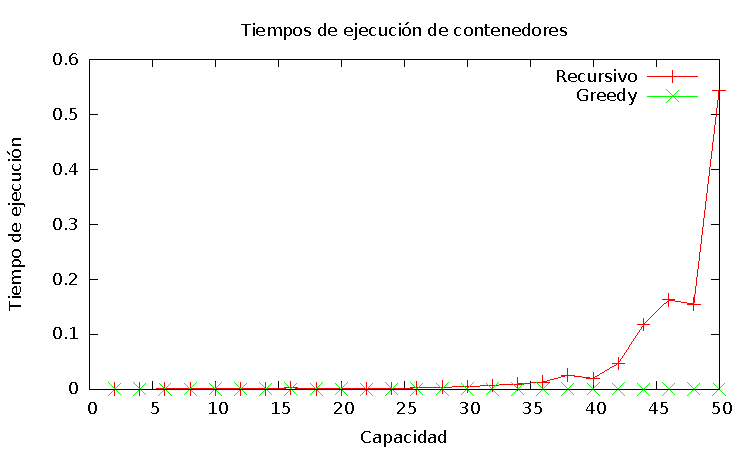
\includegraphics[width = \linewidth ]{contenedores_tiempo}
	\end{center}
\end{frame}

\begin{frame}{Comparativa}
	\begin{center}
		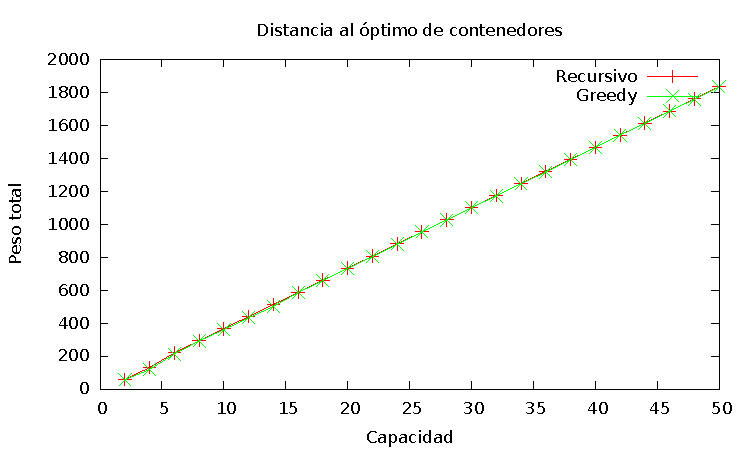
\includegraphics[width = \linewidth ]{contenedores_peso}
	\end{center}
\end{frame}

\begin{frame}{Conclusión}
	Este es un ejemplo en el que es posible que nos interese trabajar con algoritmos greedy si quisiéramos conseguir una solución rápida a un problema grande.
\end{frame}